\chapter{Introduzione}

\section{Il Corso in Breve...}

\paragraph{Obiettivi:}

\begin{itemize}
  \item Riconoscere problemi di privacy nella modellazione e nell'analisi dei dati. 
  \item Conoscenza di base su metodi per preservare la privacy.
\end{itemize}

\paragraph{Syllabus:}

\begin{enumerate}
  \item Il concetto di privacy e le leggi sulla privacy in differenti paesi. 
  \item Le sfide della privacy nell'era dei Big Data. 
  \item Sistemi di informazione. 
  \item Modelli statistici. 
  \item Attacchi alla privacy e modelli di anonimizzazione in database statistici. 
  \item Privacy differenziale. 
  \item Separazione dei dati.
\end{enumerate}

\section{Privacy e Leggi sulla Privacy}

\subsection{Che Cos'è la Privacy?}

\qs{}{Che cos'è la privacy?}

\dfn{Privacy 1}{
  La \newfancyglitter{privacy} può essere definita come il diritto a stare da soli.
}

\paragraph{Warren and Brandeis (1890), \textit{The Right to Privacy}:}

\begin{itemize}
  \item Una delle tesi più influenti nella storia americana. 
  \item GLi autori tentarono di trovare un modo di descrivere legalmente la privacy.
\end{itemize}

\nt{Esempio: il diritto di una persona a scegliere la seclusione dalle attenzioni altrui, il diritto di non essere osservati nella sfera privata.}

\dfn{Privacy 2}{
  La \newfancyglitter{privacy} può essere definita come accesso limitato alle informazioni.
}

\begin{itemize}
  \item Una persona deve essere libera di scegliere in che misura partecipare alla società senza che gli altri debbano sapere. 
  \item Godkin (1880): “nothing is better worthy of legal protection than
private life, or, in other words, the right of every man to keep his
affairs to himself, and to decide for himself to what extent they
shall be the subject of public observation and discussion.”. 
\item Bok (1989): la privacy è "the condition of being protected from
unwanted access by others—either physical access, personal
information, or attention.".
\end{itemize}

\dfn{Privacy 3}{La \newfancyglitter{privacy} può essere vista come controllo sull'informazione.}

\begin{itemize}
  \item Westin and Blom-Cooper (1970): "privacy is the claim of
individuals, groups, or institutions to determine for
themselves when, how, and to what extent information
about them is communicated to others.“. 
\item Fried (1968): "Privacy is not simply an absence of
information about us in the minds of others; rather it is the
control we have over information about ourselves.”.
\end{itemize}

\dfn{Privacy FIPS PUB 41}{
  Il diritto di un'entità ... a determinare il grado con il quale interagire con il proprio ambiente, compreso il grado con cui un'entità voglia condividere informazioni personali con gli altri.
}

\dfn{Privacy ISO}{
  Il diritto di un individuo a controllare o influenzare quali informazioni collegate a loro possono essere collezionate e salvate e da chi e a chi queste informazioni possono essere accedute.
}

\clm{}{}{
  Definizioni derivabili:
  \begin{itemize}
    \item La privacy è l'abilità di una persona di controllare la disponibilità di \fancyglitter{informaziioni} e la sua \fancyglitter{esposizione}.
    \item È collegata a essere abili a funzionare in una società \fancyglitter{anonimamente}.
  \end{itemize}
}

\paragraph{Edward Snowden files:} viene pubblicato il file contente le informazioni riguardo i dati raccolti dal NSA riguardo le chiamate di milioni di privati cittadini. 

\subsection{Perché la Privacy è Così Importante?}

\qs{}{
  Perché la privacy è così importante?
}

\paragraph{La privacy è importante perché:}


\begin{itemize}
  \item \fancyglitter{Sentimenti individuali:}
    \begin{itemize}
      \item Non confortabile: possesso dell'informazione. 
      \item Non sicuro: l'informazione può essere usata in modo improprio (furto d'identità). 
    \end{itemize}
  \item \fancyglitter{Le aziende hanno bisogno di:}
    \begin{itemize}
      \item Far si che i loro clienti si sentano al sicuro. 
      \item Mantenere una buona reputazione\footnote{Beh, visto che merda sono Twitter e META non credo gliene freghi qualcosa.}. 
      \item Proteggere sé stesse da ogni disputa legale. 
      \item Obbedire alle leggi.
    \end{itemize}
\end{itemize}

\paragraph{Tipi di privacy:}

\begin{itemize}
  \item Political privacy. 
  \item Consumer Privacy. 
  \item Medical privacy. 
  \item Private property. 
  \item Information/Data privacy.
\end{itemize}

\dfn{Data Privacy}{
  Il problema della \newfancyglitter{data privacy} emerge quando dei dati unicamente associabili a un individuo sono collezionati e salvati.
}

\paragraph{Le fonti più comuni di dati affetti da data privacy:}

\begin{itemize}
  \item Record sanitari. 
  \item Investigazioni e processi criminali. 
  \item Transazioni finanziarie. 
  \item Tratti biologici (e. g. materiale genetico). 
  \item Residenza e posizione geografica. 
  \item Geolocalizzazione. 
  \item Utilizzo del web.
\end{itemize}

\clm{}{}{
  \begin{itemize}
    \item La sfida della data privacy è trovare un modo per \fancyglitter{condividere dati} proteggendo le informazioni che permettono di identificare una determinata persona.
      \begin{itemize}
        \item Per esempio negli ospedali i dati vengono trasferiti in maniera aggregata. 
        \item L'idea di condividere i dati in forma aggregata garantisce che solo dati non identificabili sono condivisi.
      \end{itemize}
    \item La protezione legale deò diritto alla privacy \fancyglitter{cambia drasticamente a seconda della nazione}.
  \end{itemize}
}

\subsection{Privacy negli Stati Uniti}

\paragraph{La data privacy \fancyglitter{non è molto regolata} negli USA:}

\begin{itemize}
  \item Non c'è una legge che controlli tutti gli aspetti dei dati (acquisizione, collezione, trattamento e uso). 
  \item Se un'azienda colleziona dei dati (anche senza permesso) ha il diritto di utilizzarli. 
  \item Gli istituti possono informarsi sulle condizioni finanziarie di una persona (banche, assicurazioni, etc.) chiedendo report a terze parti.
  \item Ci sono alcune eccezioni:
    \begin{itemize}
      \item Dati sanitari (HIPAA). 
      \item Dati dei bambini sotto i 13 anni online (COPPA).
      \item Richieste di prestito (FCRA). 
      \item Sicurezza informatica (ECPA, PATRIOT\footnote{Nel 2001, in seguito a un certo evento terroristico.}, etc.).
    \end{itemize}
\end{itemize}

\subsection{Privacy nell'Unione Europea}

\paragraph{La data privacy nell'UE \fancyglitter{è pesantemente regolata}:}

\begin{itemize}
  \item l'articolo 8 della convenzione europea sui diritti umani (ECHR) prevede il diritto al rispetto della privacy di una persona (poter disporre di una sfera privata, una vita familiare, un domicilio e della propria corrispondenza). 
  \item La corte dei diritti umani ha dato a quest'articolo varie interpretazioni, con le seguenti eccezioni: 
    \begin{itemize}
      \item Ottenere informazioni per censimenti ufficiali. 
      \item Raccogliere impronte digitali e fotografie per attività di polizia. 
      \item Collezionare dati medici e spese personali. 
      \item Implementare sistemi di identificazione personale (un documento di identificazione).
    \end{itemize}
\end{itemize}

\nt{Spesso questa maggiore tutela della privacy viene criticata dalle aziende che la vedono come un freno al progresso.}

\paragraph{Ci sono state due ere della privacy:}

\begin{itemize}
  \item 1995-2018: Data Protection Directive (DPD). 
  \item 2018-presente: General Data Protection Regulation (GDPR\footnote{Promulgato nel 2016, ma diventato effettivo dal maggio del 2018}).
\end{itemize}

\dfn{Data Protection Directive}{
  La Data Protection Directive (DPD) fu adottata nel 1995 dal parlamento europeo:
  \begin{itemize}
    \item Come tentativo di armonizzare la protezione dei dati nell'unione europea. 
    \item Doveva essere regolamentata da leggi nazionali nel 1998.
  \end{itemize}
}

\paragraph{Gli 8 princìpi di base del DPD:}

\begin{enumerate}
  \item I dati personali devono essere processati a norma di legge e in maniera corretta. 
  \item I dati personali devono essere processati solo per certi scopi limitati. 
  \item I dati personali devono essere processati in modo adeguato, rilevante e non eccessivo. 
  \item I dati personali devono essere processati accuratamente.
  \item I dati personali devono essere trattenuti solo per il tempo strettamente necessario.
  \item I dati personali devono essere processati in accordo con i diritti del soggetto interessato. 
  \item I dati personali devono essere processati in modo sicuro. 
  \item I dati personali devono essere trasferiti solo a nazioni con una protezione adeguata. 
\end{enumerate}

\dfn{Personal Data - DPD}{
  Ogni informazione relativa a una persona identificata i identificabile. Una persona identificabile è una persona che può essere identificata, direttamente o indirettamente, in particolare identificando un particolare numero di identificazione o uno o più fattori fisici, psicologici, mentali, economici, culturali o sociali.
}

\nt{Questa definizione viene rafforzata nel GDPR.}

\dfn{Data Processing - DPD}{
  Ogni operazione o insieme di operazioni che viene effettuata su dati personali, tramite un mezzo automatizzato o meno, come la collezione, registrazione, organizzazione, immagazzinamento, adattamento o alterazione, recupero, consultazione, uso, trasmissione, disseminazione o altra distribuzione, allineamento o combinazione, blocco, cancellazione o distruzione.
}

\nt{Vengono effettuati cambiamenti minori nel GDPR.}

\dfn{Responsabile - DPD}{
  Il responsabile può essere una persona fisica o giuridica, un autorità pubblica o un ente che deve garantire l'integrità dei dati trattati.
}

\cor{Processore}{
  Il processore dei dati è una persona fisica o giuridica, un'autorità pubblica, un'agenzia o qualunque altro ente che processa i dati personali per conto del responsabile. 
}

\nt{Non ci sono cambiamenti nel GDPR.}

\paragraph{Princìpi della gestione dei dati. I dati personali non dovrebbero essere processati a meno che non riguardino queste categorie:}

\begin{itemize}
  \item \fancyglitter{Trasparenza}: il soggetto dei dati ha il diritto di essere informato da un'azienda che sta elaborando i suoi dati personali.
  \item \fancyglitter{Scopo legittimo}: i dati personali possono essere processati solo per scopi legittimi e non usati per altri scopi non pertinenti.
  \item \fancyglitter{Proporzionalità}: i dati personali processati devono essere adeguati, rilevanti e non eccessivi in relazione allo scopo per quale i dati vengono collezionati e ulteriolmente processati.
\end{itemize}

\paragraph{Trasparenza:}

\begin{itemize}
  \item Il soggetto dei dati deve dare il \fancyglitter{consenso}. 
  \item Il processamento era necessario per l'\fancyglitter{esecuzione di un contratto}. 
  \item Il processamento era necessario per \fancyglitter{assolvere un obbligo legale}. 
  \item Il processamento era necessario per \fancyglitter{proteggere gli interessi vitali} del soggetto dei dati.
  \item Il processamento era necessario per un'operazione di \fancyglitter{interesse pubblico}. 
  \item Il processamento era necessario per \fancyglitter{scopi di interesse legittimato dal controllore, eccetto quando quegli interessi sono sovrascritti dagli interessi dei diritti fondamentali e della libertà del soggetto}.
\end{itemize}

\clm{}{}{
  Il soggetto ha il diritto a:
  \begin{itemize}
    \item Accedere a tutti i dati su di lui/lei/loro. 
    \item Domandare la rettifica, cancellazione o blocco dei dati se sono incompleti, inaccurati o non sono processati come previsto dalle regole sulla protezione dei dati.
  \end{itemize}
}

\paragraph{Proporzionalità:}

\begin{itemize}
  \item I dati devono essere accurati e, quando necessario, aggiornati. 
  \item I dati non devono essere mantenuti in una forma che permette l'identificazione del soggetto per più tempo del necessario. 
  \item Gli stati membri hanno la possibilità di memorizzare i dati personali per fini statistici o scientifici. 
  \item Vengono applicate tutele aggiuntive per la gestione dei \fancyglitter{dati sensibili} (credenze religiose, opinioni politiche, salute, orientamento sessuale, gruppo etico, appartenenza a organizzazioni). 
  \item Il soggetto può sempre chiedere la cancellazione dei suoi dati usati per fini pubblicitari\footnote{Contrariamente agli stati uniti.}. 
  \item Qualunque decisione automatizzata sulla persona non deve essere fatta in maniera completamente automatica. 
  \item L'individuo può \fancyglitter{fare ricorso} su qualsiasi decisione automatica in cui vengono processati i propri dati.
\end{itemize}

\paragraph{Autorità della privacy:}

\begin{itemize}
  \item Ogni stato membro deve eleggere un'\fancyglitter{autorità di supervisione} che: 
    \begin{itemize}
      \item Deve \fancyglitter{monitorare la protezione dei dati} in quello stato membro. 
      \item Dare \fancyglitter{avvisi al governo riguardo le misure amministrative e i regolamenti}. 
      \item \fancyglitter{Iniziare procedure legali} quando il regolamento sulla protezione dei dati viene violatao.
    \end{itemize}
  \item Il \fancyglitter{controllore} deve notificare all'autorità di supervisione le seguenti informazioni:
    \begin{itemize}
      \item Il nome e l'indirizzo del controllore. 
      \item Lo scopo del processamento. 
      \item Una descrizione delle categorie dei dati del soggetto. 
      \item Il recipiente a cui i dati possono essere inotrati. 
      \item Proposte di trasferimento dei dati a stati terzi. 
      \item Una descrizione generale delle misure prese per garantire la sicurezza dei dati processati.
    \end{itemize}
  \item Le informazioni sono tenute in un \fancyglitter{registro pubblico}.
\end{itemize}

\paragraph{Leggi della privacy in Italia:}

\begin{itemize}
  \item Il DPD è stato implementato con il decreto legislativo 196/2003 (Codice in materia di protezione dei dati personali). 
  \item Inoltre il Garante per la protezione dei dati limitati doveva applicare misure appropriate in determinati campi (video sorveglianza, dati biometrici, dati sanitari, notifiche di data breach, informazioni bancarie, profili online, processamenti fatti da amministratori di sistema, processamenti a fini di marketing e profiling, pagamenti elettronici, cookies).
\end{itemize}

\dfn{General Data Protection Regulation}{
  La General Data Protection Regulation (GDPR) è un regolamento attraverso il quale l'unione europea intende aumentare la forza e unificare la protezione dei dati per tutti gli individui all'interno dell'unione europea.
}


\nt{L'obiettivo principale del GDPR è quello di offrire un controllo semplificato agli appartenenti ai paesi membri dell'unione europea.}

\dfn{Personal Data - GDPR}{
  Uguale al DPD, ma aggiunge come caratteristiche di identificazione i dati di locazion, gli identificatori online, lo stato genetico, economico e culturale.
}

\dfn{Data Processing - GDPR}{
  Uguale al DPD, ma viene inclusa la "strutturazione" dei dati processati.
}

\nt{Inoltre il GDPR include altre definizioni.}

\dfn{Pseudoanimizzazione}{
La pseudoanimizzazione è il processamento in cui i dati personali non possono più essere attribuiti univocamente a un soggetto senza informazioni aggiuntive. Le informazioni aggiuntive sono tenute separate e soggette a misure tecniche e organizzative per assicurare che i dati siano anonimi.
}

\paragraph{La pseudoanimizzazione:}

\begin{itemize}
  \item Se viene effettuata con politiche adeguate non è soggetto a controlli e penalità. 
  \item La regolamentazione non coinvolge dati usati per statistiche o ricerche. 
  \item Le politiche e le misure che raggiungono la privacy by Design e la privacy by Default sono adeguati.
\end{itemize}

\dfn{Personal Data Breach}{
  Un leak accidentale nella sicurezza  per cui il dato personale viene distrutto, perso, alterato, rubato o acceduto.
}

\paragraph{Diritti del soggetto:}

\begin{itemize}
  \item L'individuo deve dare un \fancyglitter{consenso chiaro} per il trattamento dei propri dati. 
  \item Il soggetto ha un \fancyglitter{facile accesso} ai propri dati. 
  \item Viene evidenziato il diritto alla rettifica, alla cancellazione e all'oblio\footnote{Cosa non facile, soprattutto con i social.}. 
  \item Il diritto di obiezione, incluso l'utilizzo dei propri dati per "profiling". 
  \item Il diritto alla portabilità dei dati da un servizio a un altro.
\end{itemize}

\paragraph{Privacy \fancyglitter{by Design} e \fancyglitter{by Default}:}

\begin{itemize}
  \item Viene richiesto che la protezione dati sia presente fin dall'inizio nel sistema informativo. 
  \item Le impostazioni della privacy devono essere di alto livello.
  \item La privacy deve essere presente per tutto il ciclo di vita del processamento dei dati. 
  \item Come già detto i dati personali devono essere processati solo quando è necessario per ogni specifico scopo.
\end{itemize}

\dfn{Privacy by Design - Ann Cavoukian}{
  Un approccio all'ingegneria dei sistemi che tiene in considerazione la privacy durante tutto il ciclo di vita. Si basa su 7 princìpi fondamentali:
  \begin{enumerate}
    \item Proattività, non reattività (prevenzione, non rimedio). 
    \item Privacy come impostazione di Default. 
    \item Privacy integrata nel Design. 
    \item Completamente funzionale. 
    \item End-to-end security. 
    \item Visibilità e trasparenza. 
    \item Rispetto per la privacy degli utenti.
  \end{enumerate}
}

\paragraph{Responsabilità:}

\begin{itemize}
  \item Il titolare del trattamento del dato deve dimostrare che tutte le operazioni messe in atto per garantire la sicurezza del dato siano aderenti alla legge. 
  \item È responsabilità del controllore dei dati di implementare misure effettive e di dimostrare la \fancyglitter{compliance} alle attività di processamento. 
  \item L'utente deve essere chiaramente informato riguardo le finalità del trattamento, alla legge usata come base, all'intervallo temporale del trattamento, se i dati vengono trasferiti a terze parti e se avvengono delle decisioni automatizzate. 
  \item Viene introdotto il \fancyglitter{Data Protection Officer}, un esperto tecnico del dato e legale del GDPR. 
  \item Se avvengono eventi di rischio bisogna fare un \fancyglitter{Data Protection Impact Assessments} (DPIA) per valutarne l'estensione. 
  \item La valutazione e la mitigazione del rischio sono necessarie e approvazione delle autorità nazionali di protezione dei dati (DPA) è necessario per rischi elevati. 
  \item I records delle attività di trattamento devono essere conservate in modo includere le finalità del trattamento, le categorie coinvolte e Termini previsti.  
  \item I records devono essere disponibili all'autorità di supervisione, su richiesta.
\end{itemize}

\dfn{Data Protection Officer}{
Il GDPR stabilisce la figura del Data Protection Officer (DPO), una persona con conoscenze specialistiche in materia di protezione dei dati e pratiche che dovrebbero aiutare il titolare del trattamento o l'incaricato del trattamento a monitorare conformità interna al presente regolamento. The DPO are also expected to be proficient at managing IT
processes, data security (including dealing with cyber-attacks)
and other critical business continuity issues around the holding
and processing of personal and sensitive data. 
}

\nt{
  Autorità pubbliche e imprese le cui attività principali sono trattamento regolare o sistematico dei dati personali, sono necessario per assumere un DPO.
}

\dfn{Data Breach}{
  Il controllore dei dati ha l'obbligo legale di notificare l'autorità di supervisione senza ritardi non necessari, a meno che sia improbabile che il data breach causi rischi alla libertà e ai diritti dell'individuo. C'è un massimo di 72 ore dopo aver scoperto il data breach per notificare. 
}

\paragraph{Le seguenti sanzioni possono essere imposte:}

\begin{itemize}
  \item Nel primo e non intenzionale caso di noncompliance viene emesso un avviso. 
  \item Una multa fino a 10 milioni di euro o fino al 2\% dell'annualità mondiale fatturato dell'esercizio finanziario precedente nel caso di un'impresa, se vi è stata una violazione di alcuni obblighi. 
  \item Una multa fino a 20 milioni di euro o fino al 4\% dell'annuo in tutto il mondo fatturato dell'esercizio finanziario precedente nel caso di un'impresa, se vi sono state gravi violazioni dei princìpi.
\end{itemize}

\subsection{Regolamenti Transazionali}

\begin{itemize}
  \item Safer Harbor privacy principles (fino al 2015). 
  \item EU-US Privacy Shield (2016-2020\footnote{Caduto a causa del primo governo Trump.}). 
  \item EU-US Data Privacy Framework (2023-presente).
\end{itemize}

\dfn{Safe Harbor}{
  Sviluppato tra il 1998 e il 2000 al fine di impedire alle organizzazioni private di l'UE o gli Stati Uniti dalla divulgazione accidentale o dalla perdita di informazioni personali.
}

\paragraph{Le compagnie USA che tengono dati devono aderirea questi 7 princìpi:}

\begin{enumerate}
  \item \fancyglitter{Notifica}: gli individui devono essere informati che i loro dati stanno venendo collezionati e come verranno usati. 
  \item \fancyglitter{Scelta}: gli individui possono scegliere di rimuovere i propri dati rinunciando ai servizi\footnote{Google merda.}.
  \item \fancyglitter{Trasferimento}: la trasmissione dei dati a terzi può avvenire solo ad altri organizzazioni che seguono principi di protezione dei dati adeguati. 
  \item \fancyglitter{Sicurezza}: bisogna evitare la perdità di informazioni collezionate. 
  \item \fancyglitter{Data Integrity}: i dati devono essere rilevanti e affidabili per lo scopo per cui sono raccolti. 
  \item \fancyglitter{Accesso}: gli individui devono essere in grado di accedere, correggere e cancellare i propri dati. 
  \item \fancyglitter{Applicazione}: devono esistere mezzi efficaci per far rispettare queste norme.
\end{enumerate}

\paragraph{Breve storia di Safe Harbor:}

\begin{itemize}
  \item Nel 2000 la Commissione europea ha deciso che il principi degli Stati Uniti erano conformi alla direttiva dell'UE (la cosiddetta "Decisione Safe Harbor"). 
  \item Dopo che un cliente si è lamentato del fatto che i suoi dati di Facebook non erano sufficientemente protetti la corte di giustizia della commissione europea, nel 2015, dichiara la decisione di Safe Harbor invalida.
  \item La Commissione ha tenuto ulteriori colloqui con gli Stati Uniti autorità competenti verso "un quadro rinnovato e solido per flussi di dati transatlantici". 
  \item La Commissione europea e gli Stati Uniti hanno convenuto di istituire un nuovo quadro per i flussi transatlantici di dati il 2 febbraio 2016, noto come "EU-US Privacy Shield". 
\end{itemize}

\dfn{EU-US Privacy Shield}{
  Lo scudo UE-USA per la privacy è un quadro per gli scambi transatlantici di dati per finalità commerciali tra l'Unione Europea e gli Stati Uniti. Uno dei suoi scopi è quello di consentire alle aziende statunitensi di ricevere più facilmente dati provenienti da entità dell'UE ai sensi delle leggi sulla privacy dell'UE volte a proteggere i cittadini dell'unione europea. 
}

\clm{}{}{
  \begin{itemize}
    \item La Commissione europea ha adottato il quadro il 12 luglio 2016 ed è entrato in vigore lo stesso giorno. 
    \item Il presidente degli Stati Uniti Donald Trump ha firmato un ordine esecutivo intitolato "Enhancing Public Safety", in cui si afferma che le protezioni della privacy degli Stati Uniti non saranno estese oltre i cittadini o residenti statunitensi. 
    \item Nel luglio 2020 lo scudo UE-USA per la privacy è stato abrogato dalla Corte europea giustizia in quanto non forniva tutele adeguate ai cittadini dell'UE rispetto allo Snooping governativo americano\footnote{In poche parole gli americani si comportano da americani.}.
  \end{itemize}
}

\dfn{AI Act}{
  La legge sull'IA mira a garantire che i sistemi di IA utilizzati nell'UE siano sicuri, trasparenti e rispettosi diritti fondamentali.
}

\paragraph{L'AI Act classifica i sistemi di IA in base al livello di rischio che rappresentano:}

\begin{itemize}
  \item \fancyglitter{Rischio inaccettabile}: i sistemi di IA che rappresentano una chiara minaccia per la sicurezza o i diritti fondamentali sono vietato. Ciò include i sistemi che implementano tecniche subliminali per manipolare il comportamento, sfruttare le vulnerabilità di gruppi specifici o abilitare il punteggio sociale da parte dei governi.
  \item  \fancyglitter{Alto rischio}: sistemi di intelligenza artificiale utilizzati in aree critiche come la sanità, l'istruzione, l'occupazione, il diritto l'applicazione delle norme e i servizi essenziali sono soggetti a obblighi rigorosi. Questi includono rigorosi valutazioni dei rischi, misure di governance dei dati, supervisione umana e monitoraggio continuo per garantire la conformità. 
  \item \fancyglitter{Rischio limitato}: i sistemi di intelligenza artificiale a rischio limitato, come i chatbot e i deepfake, sono soggetti a obblighi di trasparenza. I fornitori e i distributori devono informare gli utenti che stanno interagendo con un sistema di intelligenza artificiale. 
  \item \fancyglitter{Rischio minimo}: la maggior parte dei sistemi di intelligenza artificiale, come i videogiochi abilitati all'intelligenza artificiale o i filtri antispam, cadono rientrano in questa categoria e sono in gran parte non regolamentate, incoraggiando l'innovazione e lo sviluppo.
\end{itemize}

\paragraph{Tutti i providers di modelli di AI devono:}

\begin{itemize}
  \item Fornire documentazione tecnica e istruzioni. 
  \item Rispettare la direttiva europea sul copyright. 
  \item Pubblicare un sommario dei dati usati per il training. 
  \item Condurre valutazioni e test (anche di tipi "adversarial"\footnote{Per portare il sistema in errore.}. 
  \item Assicurare misure di cybersecurity adeguate.
\end{itemize}

\nt{Questo copre la parte legale di assegnamento delle responsabilità in campo giuridico.}

\paragraph{Obblighi:}

\begin{itemize}
  \item \fancyglitter{Sviluppatori:} entità che sviluppano sistemi ad alto rischio, devono assicurarsi che i datasets siano di alta qualità, mantenere documentazione tecnica e sviluppare sistemi con livelli di sicurezza, robustezza e sicurezza.
  \item \fancyglitter{Utilizzatori:} chi utilizza sistemi ad alto rischio deve monitorare le performance e ridurre/mitigare i rischi con la presenza umana.
\end{itemize}

\clm{}{}{
  \begin{itemize}
    \item L'AI act prevede un board europeo che monitori l'intelligenza artificiale.
    \item Controlla le implementazioni negli stati membri.
    \item Forzano l'aderenza alla legge.
  \end{itemize}
}

\dfn{Digital Service Act (2018)}{
  Regola i servizi online. Sono 44 articoli e 128 misure che coprono le seguenti aree:
  \begin{itemize}
    \item Demonetizzazione: riduzione degli incentivi finanziari per leakers e disinformatori. 
    \item Trasparenza nella pubblicità politica. 
    \item Integrità dei servizi: riduzione di account fake, deepfake, amplificazione dovuta a bots, disinformazione, etc. 
    \item Fact-checking\footnote{Non se il tuo cognome è Musk.}.
  \end{itemize}
}

\section{La Privacy al Tempo dei "Big Data"}

\subsection{La Privacy sotto Attacco}

Nel 1996, il 24\% degli americani ha subito un'invasione della sua privacy. Questo tema rientra nel più ampio spettro del tema: privacy vs. convenienza. 

\begin{center}
+ PRIVACY $\Leftrightarrow$ - COMODITÀ

  + COMODITÀ $\Leftrightarrow$ - PRIVACY
\end{center}

\nt{Questo trade-off è il risultato di ignoranza e di una politica di conformismo e indifferenza.}

\paragraph{Violazione della privacy, secondo alcune persone:}

\begin{itemize}
  \item Chiamate di basso livello per ottenere l'identificatore univoco nei chip intel. 
    \item Database delle immagini dei guidatori negli USA. 
    \item Utilizzo dei dati di Facebook. 
    \item Scandali del NSA. 
    \item Cambridge Analytica e scandali di Facebook.
\end{itemize}

\nt{Negli anni si sta verificando un sempre maggiore raccoglimento di dati personali: carte di credito, registri di chiamate, dati sulla sanità, emails, account social, DNA, etc.}

\dfn{Big Data}{
Il termine Big Data si riferisce all'acquisizione e all'analisi di enormi collezioni di informazioni, talmente grandi che fino a poco tempo fa la tecnologia per analizzarli non esisteva.
}

\cor{Legge delle Conseguenze Inattese}{
La legge delle conseguenze inattese è un fenomeno frequentemente osservato per cui ogni azione ha risultati che non fanno parte delle intenzioni dell'attore. Le conseguenze possono essere positive, neutrali o negative.
}

\subsection{Deanonimizzazione}

I dati vengono raccolti in modo che siano anonimizzati (vedremo in un successivo capitolo come). Però a volte si può bypassare questa anonimizzazione, com'è successo nel caso di Netflix nel 2006:

\begin{itemize}
  \item Si potevano incrociare due datasets (uno anonimizzato per una challenge di netflix e l'altro non anonimizzato riguardante i rating dei film). 
  \item Così facendo, conoscendo 6-8 valutazioni di film e date, si potevano identificare unicamente gli utenti con una probabilità del 90\%. 
  \item Non si può sempre anonimizzare i dati semplicemente rimuovendo gli identificatori. 
  \item Si ha una vulnerabilità aggregando dati da sorgenti diverse (fig: \ref{fig:ae}).
\end{itemize}

\begin{figure}[h]
    \centering
    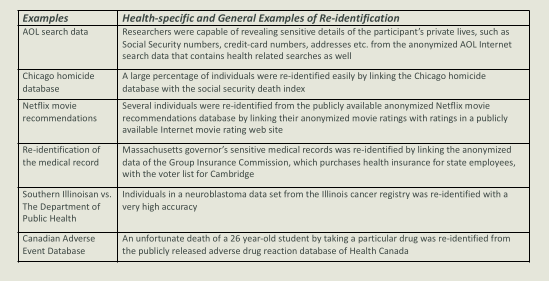
\includegraphics[scale=0.65]{01P/re-id.png}
    \caption{Esempi di re-identificazione.}
    \label{fig:ae}

  \end{figure}

\subsection{Data Breach}

\paragraph{Cause comuni di data breaches:}

\begin{itemize}
  \item Credenziali compromesse. 
  \item Servizi malconfigurati. 
  \item Vulnerabilità software.
\end{itemize}

\nt{Un caso emblematico italiano è il data breach avvenuto a danni dell'INPS durante il governo Renzi (fig: \ref{fig:db}).}

\begin{figure}[h]
    \centering
    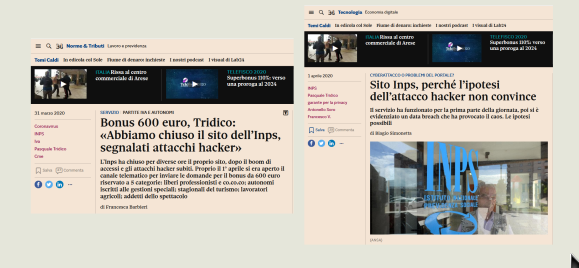
\includegraphics[scale=0.65]{01P/db.png}
    \caption{INPS data breach.}
    \label{fig:db}

  \end{figure}
\qs{}{Ma qual è il costo di un data breach?}

\begin{itemize}
  \item I data breach sono molto costosi, sia in termini di valore dei dati che di credibilità. 
  \item Si stima che il costo per i cittadini dei propri dati sia tra 1000\$ e 3000\$
  \item Stefano Rodotà lega il concetto di privacy alla dignità attribuendo un costo immenso alla perdità dei propri dati personali.
\end{itemize}










